\scanpage{87}

\uline{norme de \unsure{Schatten}} $N(x_1,-x_n)$ \uline{satisfait \deleted{\unsure{à la|la}}\inserted{à \deleted{de} la} condition envisagée} \uline{dans l'énoncé du \deleted{corollaire 1}}\inserted{Th. 1, 2°} \deleted{\unsure{rappelé ci-dessus}}\inserted{pour la fonction $f$. On en conclut,} si $(\rho_i)$ \deleted{$\unsure{\rho(\sigma_i|\rho(x)}$} et $(\sigma_i)$ sont comme dans le th. :

\reversemarginpar
\margin{\textcircled{\unsure{11|13}} $N(\rho_1,-\rho_n)\leq N(\sigma_1,-\sigma_n)$ et plus généralement, compte tenu d'une remarque qui précède, et en \deleted{\unsure{pour que}} posant pour $1\leq k\leq n$ : $N(\rho_1,-\rho_k)=N(\rho_1,-\rho_k,0-0)$ \textcircled{12} $N(\rho_1,-\rho_k)\leq N(\sigma_1,-\sigma_k)$ pour $1\leq k\leq n$}
\normalmarginpar

\deleted{De =, \unsure{si on sait} que la fonction $(e^{t_i})^p$ étant une \unsure{fonction convexe}} \deleted{\inserted{\uline{la fonction} $f(r_1,-r_n)=r_1^p\unsure{-|+}+r_n^p$,} \uline{$p$ est un nb réel quelconque, satisfait aux \deleted{\unsure{conditions}}} \uline{conditions} \deleted{\unsure{du lemme}} \uline{envisagées dans le corollaire 1}, \deleted{\unsure{donc} \uline{dans l'hypothèse b, et = \deleted{\unsure{à toutes les}}\inserted{\unsure{on a|aux|cas a}} conditions envisagées} \uline{dans l'hypothèse a.}}}

Par suite, \deleted{\unsure{sous la condition,}}\inserted{sous les conditions} de l'hypothèse b, \deleted{\unsure{on}} $(\prod_1^M\rho_i\leq\prod_1^M\sigma_i\ \inserted{\text{pour }1\leq M\leq n},\ \prod_1\rho_i=\prod_1^n\sigma_i\ne0)$ on aura

\[
\begin{array}{ll}
(\unsure{1|9}5) & \displaystyle\sum_1^n\rho_i^p\leq\sum_1^n\sigma_i^p\qquad(p\text{ réel.})
\end{array}
\]

\deleted{\unsure{et dans le cas a|et sous les cond}} \inserted{et si $p\geq0$,} on aura, pourvu que $\prod_1^M\rho_i\leq\prod_1^M\sigma_i$ pour \inserted{$1\leq M\leq n$}, \deleted{on aura}

\[
\begin{array}{ll}
\deleted{\unsure{(12)}}\inserted{(16)} & \displaystyle\sum_1^k\rho_i^p\leq\sum_1^k\sigma_i^p\qquad(p\geq0,\ \deleted{\unsure{et}} k=1-n.)
\end{array}
\]

\deleted{Remarquons d'ailleurs que 2 \unsure{systèmes|suites} \inserted{\deleted{\unsure{positifs}}} $(\rho_i),(\sigma_i)$ \inserted{positifs} \unsure{donnés|formant}, \deleted{\unsure{dès}} satisfaisant aux inégalités (16), pour \deleted{tout} $k$, et \deleted{tout} $p$ \unsure{entier|réel} $\geq0$, on peut \uline{\unsure{propriété}} \unsure{réciproque|réciproquement}}

\deleted{\unsure{Nous pouvons arriver à}}

\reversemarginpar\margin{\uline{Th 2}}\normalmarginpar
(\uline{Premier Théorème de convexité dans les espaces de Hilbert})

\reversemarginpar
\margin{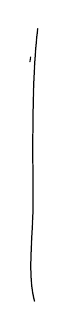
\begin{tikzpicture}[x=1cm,y=1cm]
\draw[line width=.45pt] (0,.02) .. controls (-.08,-.65) and (-.06,-1.5) .. (-.06,-2.3) .. controls (-.08,-2.8) and (-.12,-3.15) .. (-.04,-3.45);
\draw[line width=.4pt] (-.09,-.34)--(-.10,-.41);
\end{tikzpicture}}
\normalmarginpar
\deleted{\unsure{1)}} Soit $u$ un opérateur compact dans un espace de Hilbert, soit \deleted{$\varphi$ \unsure{la suite}} $f$\inserted{$(r_1,-r_n)$} une fonction \inserted{continue et symétrique} de $n$ arguments $r_i\geq0$, croissante \unsure{par r.|p. r.} à \unsure{chaq.|chaque} $r_i$, et telle que $f(e^{t_1},\mathord{-}\,\mathord{-},e^{t_n})$ soit fonction convexe de $(t_i)\in R^n$. Alors on a (\deleted{\unsure{en prenant} $\rho_i$} (avec les notations indiquées au N° \unsure{1|?|3}, avant la prop 3)

\[
\begin{array}{ll}
(17) & \displaystyle f(|\lambda_1|,\mathord{-}\,\mathord{-},|\lambda_n|)\leq f(\rho_1,\mathord{-}\,\mathord{-}\rho_n)
\end{array}
\]

Il suffit en effet de conjuguer le corollaire 1 du lemme 1 \deleted{\unsure{cas de}} (hypothèse a), avec le N° \unsure{?|1|2}, prop 3 ; corollaire 2. -- En particulier

\uline{Corollaire 1} Si $f\deleted{\unsure{(r)|(\rho)}}$ est une fonction \deleted{\unsure{croissante|convexe}}\inserted{continue} croissante de $r\geq0$ telle que $f(e^t)$ soit convexe, et $u$ un op. compact dans un espace de Hilbert, on a

\reversemarginpar\margin{88}\normalmarginpar

